\chapter{DEMO HỆ THỐNG}
\label{ch:15}

\section{Kịch bản demo hệ thống thực tế}
Trình diễn luồng đăng nhập phân quyền, nhập kho hàng loạt, cảnh báo LED đỏ khi cạn tồn và hỏi đáp thông minh qua AI Chat Console.

\section{Hình ảnh minh chứng các giao diện SaaS Dashboard, Sản phẩm và AI Hub}
Hệ thống vận hành thực tế tại cổng 3000 với đầy đủ giao diện minh chứng (giữ nguyên màu sắc thực tế làm bằng chứng kỹ thuật):

\begin{figure}[htbp]
    \centering
    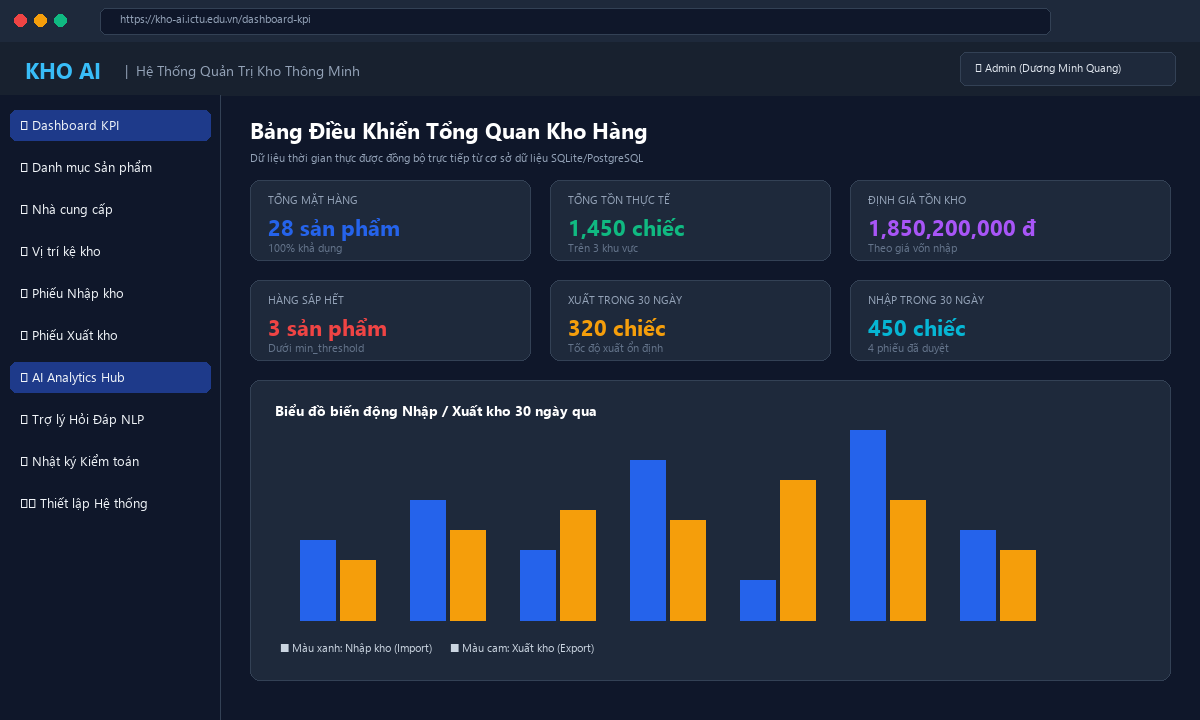
\includegraphics[width=0.92\textwidth]{11_screenshot_dashboard.png}
    \caption{Giao diện SaaS Dashboard tổng quan và 6 thẻ chỉ số KPI kho}
    \label{fig:screenshot_dashboard}
\end{figure}

\begin{figure}[htbp]
    \centering
    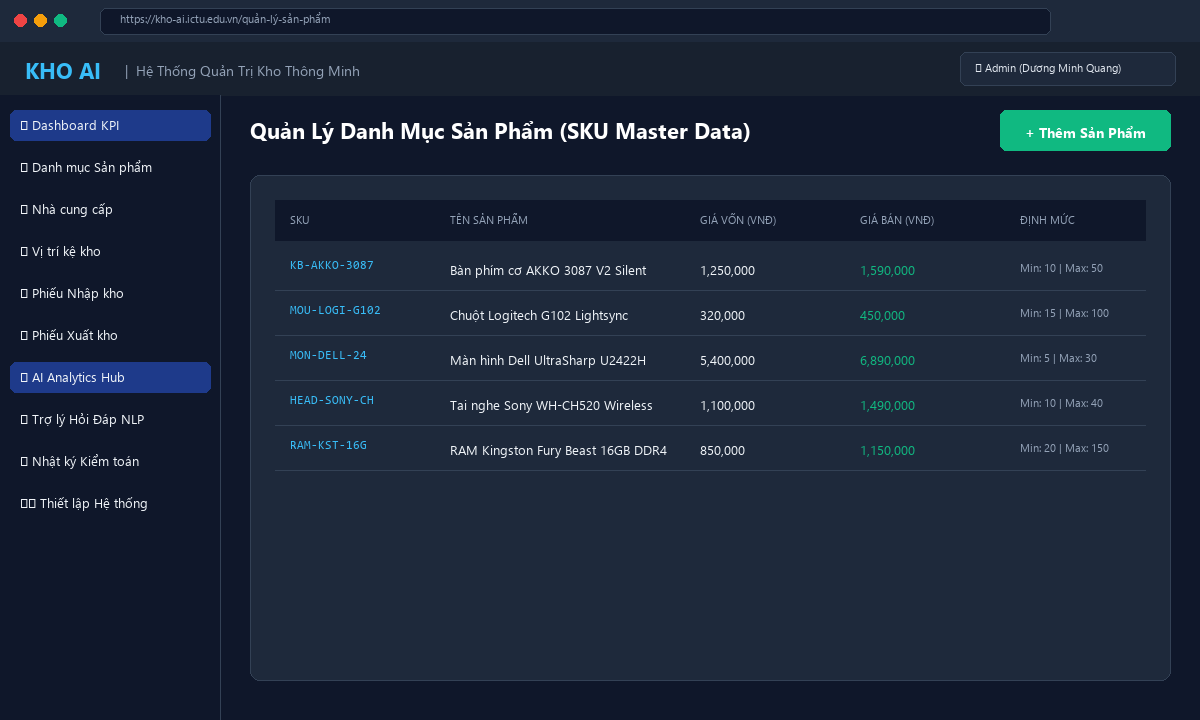
\includegraphics[width=0.92\textwidth]{12_screenshot_products.png}
    \caption{Giao diện Quản lý Danh mục Sản phẩm và Smart Table Renderer}
    \label{fig:screenshot_products}
\end{figure}

\begin{figure}[htbp]
    \centering
    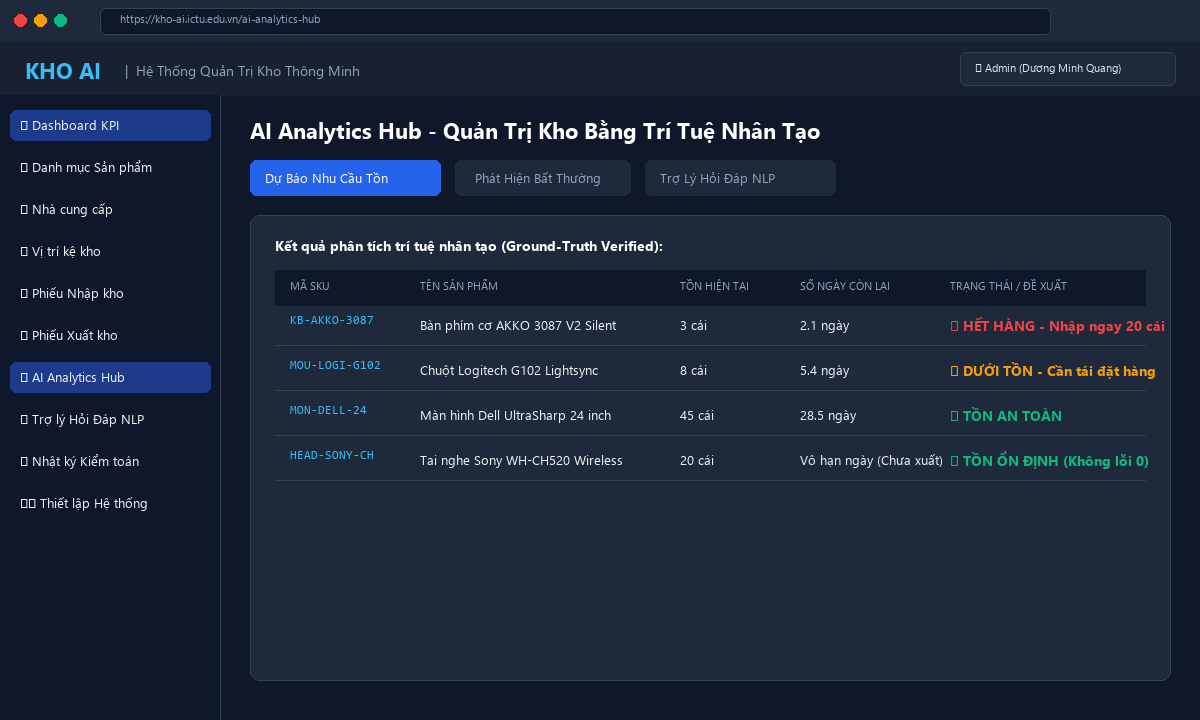
\includegraphics[width=0.92\textwidth]{13_screenshot_ai_report.png}
    \caption{Giao diện AI Analytics Hub (Dự báo cạn tồn \& Phát hiện dị biệt Z-score)}
    \label{fig:screenshot_ai_report}
\end{figure}

\begin{figure}[htbp]
    \centering
    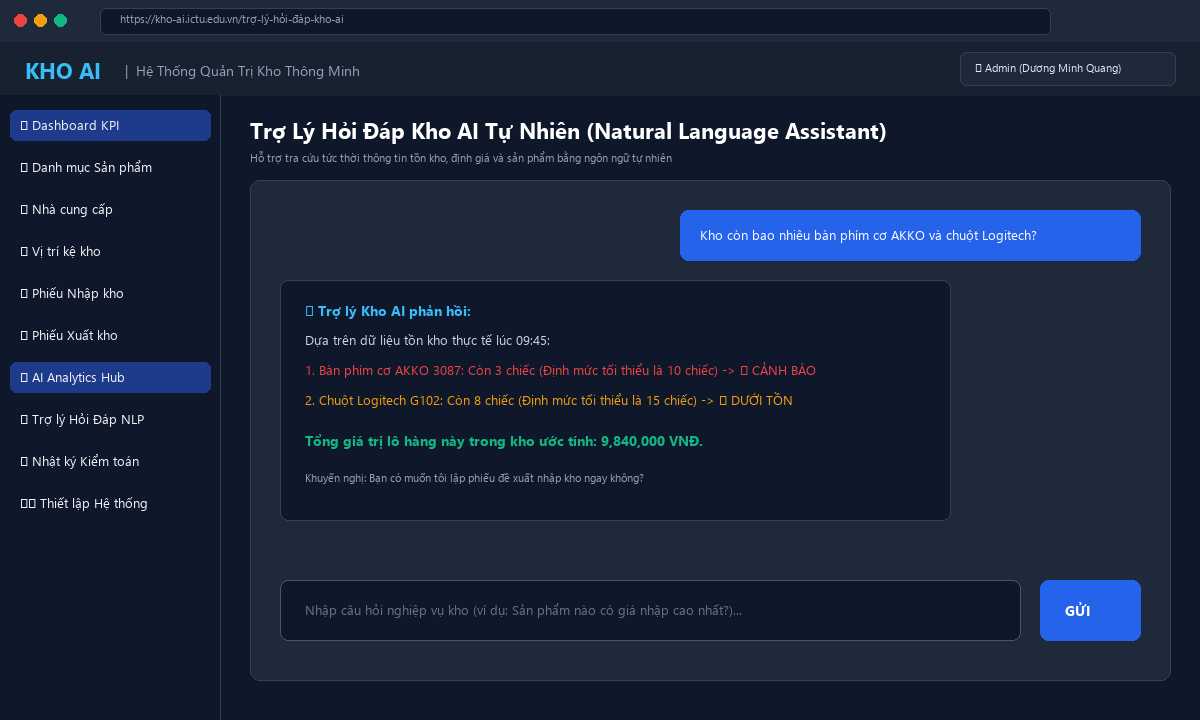
\includegraphics[width=0.92\textwidth]{14_screenshot_ai_assistant.png}
    \caption{Giao diện Trợ lý Hỏi Đáp Kho AI Tự Nhiên (AI Chat Console)}
    \label{fig:screenshot_ai_assistant}
\end{figure}
